%%%%%%%%%%%%%%%%%%%%%%%%%%%%%%%%%%%%%%%%%
% Short Sectioned Assignment
% LaTeX Template
% Version 1.0 (5/5/12)
%
% This template has been downloaded from:
% http://www.LaTeXTemplates.com
%
% Original author:
% Frits Wenneker (http://www.howtotex.com)
%
% License:
% CC BY-NC-SA 3.0 (http://creativecommons.org/licenses/by-nc-sa/3.0/)
%
%%%%%%%%%%%%%%%%%%%%%%%%%%%%%%%%%%%%%%%%%

%----------------------------------------------------------------------------------------
%	PACKAGES AND OTHER DOCUMENT CONFIGURATIONS
%----------------------------------------------------------------------------------------

\documentclass[12pt,a4paper]{report}

\usepackage[T1]{fontenc} % Use 8-bit encoding that has 256 glyphs
\usepackage{fourier} % Use the Adobe Utopia font for the document - comment this line to return to the LaTeX default
\usepackage[english]{babel} % English language/hyphenation
\usepackage{amsmath,amsfonts,amsthm} % Math packages

\usepackage{lipsum} % Used for inserting dummy 'Lorem ipsum' text into the template

\usepackage{sectsty} % Allows customizing section commands
\allsectionsfont{\centering \normalfont\scshape} % Make all sections centered, the default font and small caps

\usepackage{fancyhdr} % Custom headers and footers

% use for graph
\usepackage{graphicx} 
\usepackage{subfigure}
\usepackage{caption}
\usepackage{float} 
\usepackage{url}
\usepackage[colorlinks,linkcolor=blue]{hyperref}
\usepackage{svg}
\usepackage{indentfirst} %每段的首行缩进
\hypersetup{
    colorlinks=true,
    linkcolor=blue, % 设置链接颜色为蓝色
    urlcolor=blue, % 设置网址颜色为蓝色
    citecolor=black
}

\usepackage{url}
\usepackage{graphicx}
\usepackage{listings}
\usepackage{xcolor}
\usepackage{amsmath}



\setlength{\abovecaptionskip}{10pt} % 设置图注上方的间隔为5pt
\setlength{\belowcaptionskip}{10pt} % 设置图注下方的间隔为-10pt


\begin{document}
% \maketitle % Print the title


\begin{titlepage} \vspace{1cm}

    \begin{center}
    \textbf{\Huge Modelling Biological Neural Networks}
    \end{center}
    
    \vspace{1.5cm}
    
    \begin{center}
    \textbf{\LARGE Ananthakrishnan Sumedan \\ Kai Deng \\ Laurel Dsouza }{\LARGE\par}
    \end{center}
    
    \vfill{}
    
    \begin{center}
    {\Large AM3064/AM6015 Written Report}
    \par\end{center}
    
    \vspace{1cm}
    
    \begin{center}
    \Large{School of Mathematical Sciences \\
    University College Cork \\
    Ireland \\
    6 April 2024}
    \end{center}
    
\end{titlepage}

This report is wholly the work of the author, except where explicitly
stated otherwise. The source of any material which was not created
by the author has been clearly cited. \\
\medskip{}

Date: 6 April

\medskip{}

Signature: Ananthakrishnan Sumedan, Kai Deng, Laurel Dsouza


\tableofcontents{}

\chapter{Author Contribution}



\begin{enumerate}
    \item[] \textbf{Ananthakrishnan Sumedan}
    \begin{enumerate}
        \item Part 4 Dynamics Of Neuron.   
    \end{enumerate}
\end{enumerate}


\begin{enumerate}
    \item[] \textbf{Kai Deng}
    \begin{enumerate}
        \item Part 1 Background Concept. 
        \item Part 2 Modelling History.
        \item Part 6 Applications.
        \item Initiated the GitHub repository for team coorporation.
        \item Initiated local VSCode LaTeX environment and shared how to configure it via Zoom meeting.
        \item Find a suitable PPT template for team and check the slides.
        \item Merge the report.
    \end{enumerate}
\end{enumerate}

\begin{enumerate}
    \item[] \textbf{Laurel Dsouza}
    \begin{enumerate}
        \item Part 3 Hodgkin-Huxley Model.
        \item Part 6 Code Python Implementation.
    \end{enumerate}
\end{enumerate}




\clearpage

\chapter{Background Concept}
\section{Anatomy of a Neuron}
Neurons, the fundamental units of the brain's complex machinery, are comprised mainly of water, ions, amino acids, and proteins, boasting remarkable electrochemical properties. These diminutive entities play a pivotal role in the brain's operations. The core of our cognitive experiences, including our sensory perceptions, memories, and thought processes, stems from the fluid exchange of salts across the neuron's bi-lipid membranes and the synaptic interactions between neurons.

\begin{figure}[H]
    \centering
    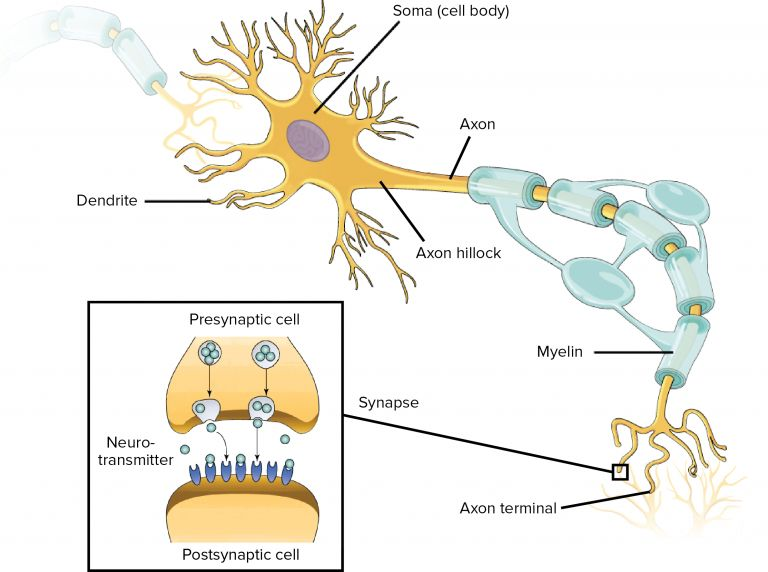
\includegraphics[width=0.7\textwidth]{./data/neural.jpg}
    \caption{Anatomy of the neuron}
    \label{fig:my_picture}
    \vspace{1pt} % Vertical space, optional
    \small{Source: Source:“Neurons and glial cells” by OpenStax College, Biology CC BY-NC-SA 3.0 License.}
\end{figure}

These neurons receive signals through synapses, which are intricately located along their dendritic trees, extensive structures characterized by their complex branching. A prime example of such complexity is seen in the Purkinje cell, notable for its ability to form up to 100,000 synaptic connections with other neurons. Dendrites, the neuron's signal-receiving extensions, are dotted with dendritic spines. These spines are crucial contact points for synaptic interaction with other neurons.

The signals collected by the dendrites are channeled towards, and converge at, the soma, or the cell body. This central part of the neuron contains the nucleus and other standard organelles found in cells, serving as a hub for signal integration.

From the soma, the axon hillock emerges, giving rise to the axon. This structure extends to form connections with other neurons at synapses, enabling rapid signal transmission over long distances without loss of signal quality. Myelination, or the presence of insulating sheaths along the axon, accelerates signal transmission by allowing electrical impulses to hop from one insulated segment to another. This ensures that the signal within the axon remains robust and unaltered, operating on an 'all-or-nothing' basis — a concept we'll explore in more depth moving forward.



\section{Physiology of a Neuron}

Understanding neurons involves delving into their unique physiological properties — their cellular functionalities. The action potential stands out as a critical feature, enabling the transmission of information across extensive distances efficiently, without diminishing the signal's strength.

Neurons exist within an aqueous extracellular environment, rich in salts and proteins. The dynamic exchange of salts entering and exiting the cell, alongside the varying salt concentrations, serve as the foundational mechanism for the neuron's exceptional functions. This process is primarily facilitated by sodium-potassium pumps, which expel sodium from the cell while importing potassium, resulting in a higher concentration of sodium externally and a lower concentration of potassium outside compared to inside the neuron.

The phenomenon of the action potential is a distinct, rapid fluctuation of the neuron's membrane potential, characterized by a swift rise (depolarization) followed by a decline (repolarization). This process adheres to an all-or-nothing rule; the occurrence of an action potential in one section of the neuron's membrane triggers a successive wave of potentials along the neuron, culminating at the axon terminal. Notably, action potentials typically do not revert to previous sections as electrochemical forces swiftly hyperpolarize the membrane area post-activation, causing the involved channels to close and temporarily inactivate.

Action potentials are generated through the orchestrated movement of different ions across the cell's membrane via specific channels, coupled with the channels' timely activation and deactivation. This detailed sequence of events underpins the typical unfolding of an action potential, highlighting the complex ionic interactions and channel dynamics essential for neuronal signaling.
\begin{figure}[H]
    \centering
    \begin{minipage}[b]{0.45\textwidth}
      \centering
      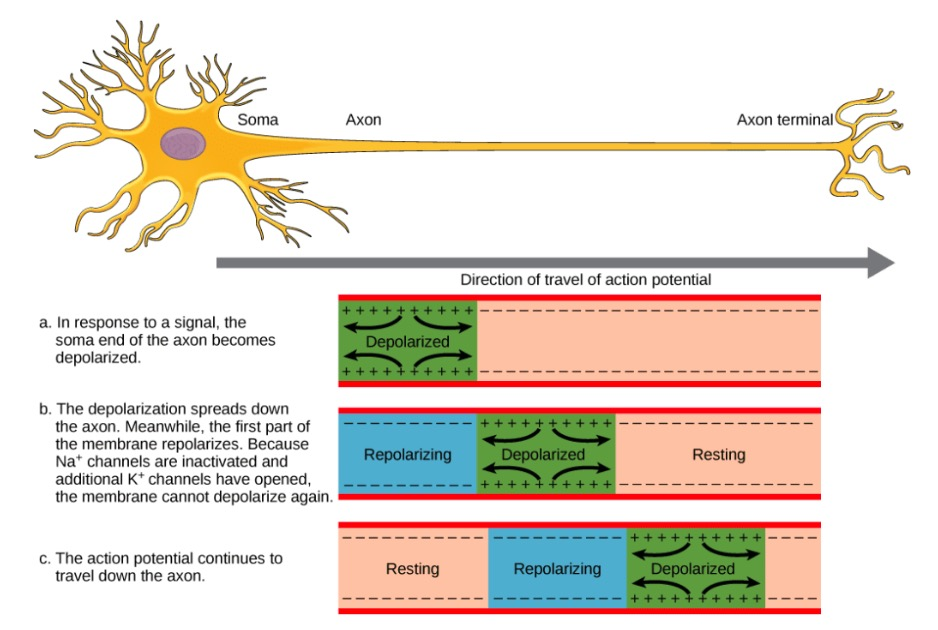
\includegraphics[width=\textwidth]{./data/propagation-of-nerve-impluse.jpg}
      \caption{Propagation of nerve impluse}
      \label{fig:exampleA}
      \vspace{1pt} % Vertical space, optional
      \small{Source: \href{https://opentextbc.ca/biology/chapter/16-2-how-neurons-communicate/}{Opentex}}
    \end{minipage}
    \hfill
    \begin{minipage}[b]{0.45\textwidth}
      \centering
      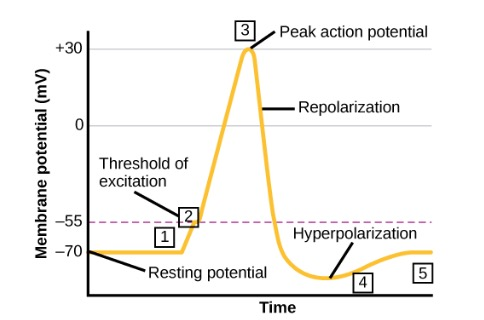
\includegraphics[width=\textwidth]{./data/neuronal-action-potential.jpg}
      \caption{Neuronal action potential}
      \label{fig:exampleB}
      \vspace{1pt} % Vertical space, optional
      \small{Source: \href{https://opentextbc.ca/biology/chapter/16-2-how-neurons-communicate/}{Opentex}}
    \end{minipage}
\end{figure}

\begin{itemize}
    \item \textbf{Equilibrium State:} The resting membrane potential of a neuron hovers around \(-70\) mV, aligning closely with the Nernst equilibrium for \( E_{K^+} \approx -75 \). In this state, there is no net movement of ions, as the influx and efflux of currents are in equilibrium.
    \item \textbf{Membrane Depolarization:} Excitatory inputs cause the neuron's membrane to depolarize. This triggers the activation of rapid voltage-gated \( Na^+ \) channels, allowing \( Na^+ \) to enter and elevate the membrane potential. Following this, the more lethargic \( K^+ \) channels open, permitting \( K^+ \) to exit and lower the membrane potential.
    \item \textbf{Signal Amplification:} With increased stimulation, a predominance of \( Na^+ \) channels over \( K^+ \) channels activates, creating a cascade where the entry of \( Na^+ \) prompts further activation of \( Na^+ \) channels.
    \item \textbf{Membrane Repolarization:} As the membrane potential approaches \( Na^+ \)'s Nernst Equilibrium with sodium channels fully open, the delayed \( K^+ \) channels overtake the \( Na^+ \) dynamics, leading to repolarization. Concurrently, \( Na^+ \) channels enter an inactive state.
    \item \textbf{Beyond Equilibrium - Hyperpolarization:} With \( K^+ \) channels remaining open while \( Na^+ \) channels are inactivated, the membrane potential momentarily falls below the equilibrium level, nearing the \( K^+ \) Nernst equilibrium.
    \item \textbf{Period of Refractoriness:} Following an action potential, \( Na^+ \) channels require time to reset, rendering them temporarily non-responsive. This phase, where \( Na^+ \) channels are effectively inoperative, is termed the absolute refractory period, during which no stimulus can provoke a spike. Conversely, the phase where a sufficiently strong stimulus can induce a spike, due to a number of \( Na^+ \) channels being inactivated, is known as the relative refractory period.
\end{itemize}


\section{Spike train}

Spike train represent the fundamental mode of communication among neurons. Commonly, spikes are conceptualized as instantaneous occurrences, while sequences of spikes are viewed as series of such events. The neural response can be mathematically represented as:

\begin{equation}
    \rho(t) = \sum_{i=1}^{k} \delta(t-t_i)
\end{equation}

Here, the representation utilizes the Dirac delta function to symbolize an impulse, ideal for enumerating discrete events:

\begin{equation}
    \delta(t) = \begin{cases} 1 & \text{if } t = 0, \\ 0 & \text{otherwise} \end{cases}
\end{equation}

For analytical purposes, it's often presumed that spike trains emanate from stochastic processes. By treating spikes as mutually independent events, one can model these trains through a Poisson process. This model provides the likelihood of observing n spikes within a time interval $\Delta T$:

\begin{equation}
    P\{n \text{ spikes occur in } \Delta t\} = \frac{(rt)^n}{n!} \exp(-rt)
\end{equation}

To simulate spikes under a Poisson point process, generate a random value r within a narrowly defined time frame, ensuring the occurrence of no more than one spike, and evaluate if $r < firingRate \Delta T$. It's crucial, however, to ensure that $firingRate\Delta T < 1$.

\section{Biological Neural Networks}
Biological neural networks constitute intricate arrangements of neurons and their synaptic connections within living organisms, fundamental to the processing and relay of information, facilitating perception, decision-making, and actions. The computational modeling of these networks strives to mimic their architecture and operational principles, offering insights into the mechanisms through which neural processing culminates in elaborate cognitive functions and behaviors. Gaining a deeper comprehension of neuronal functions and the principles of neural computation holds the potential to influence the development of novel information processing systems and advancements in artificial intelligence.






\chapter{Modelling History}

\section{The M-P model}
From the late 19th century, when the Spanish anatomist Cajal laid the groundwork for neuron theory, the biological traits and associated electrical characteristics of neurons have gradually been unveiled. In 1943, the foundational M-P neuron model was introduced in the publication "Logical Activities of Thoughts Contained in Neural Activities" \cite{Mcculloch1854LOGICALCALCULUSIDEAS}, a collaborative effort by American psychologists W.S. McCulloch and mathematician W.A. Pitts.

\begin{figure}[H]
    \centering
    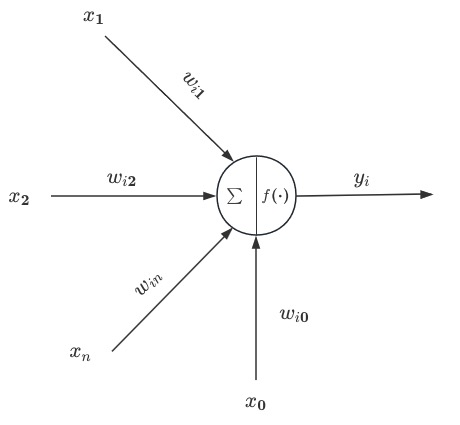
\includegraphics[width=0.6\textwidth]{./data/M-P.jpg}
    \caption{Schematic diagram of the M-P model of neurons}
    \label{fig:my_picture}
    \vspace{1pt} % Vertical space, optional
\end{figure}

In the diagram, the notation $x_i$, numbering 1, 2, ..., denotes the incoming signals from other neurons linked to the neuron in question, $w_{ij}$ signifies the synaptic weight or strength of the connection from neuron j to neuron i, and $\theta_i$ indicates the threshold or bias necessary for neuron i's activation, with f representing the activation or transfer function. The neuronal output $y_i$ is depicted by the following equation:

\begin{equation}
    y_i = f(\sum_{j=i}^{n} w_{ij}x_j-\theta_i)
\end{equation}

This framework positions neurons as logical computational units, paving the way for advanced neural network theoretical exploration. The M-P model, offering a mathematical abstraction of how biological neurons process information, serves as a cornerstone for further research in neural networks. Drawing inspiration from threshold theories related to nerve impulses, it has laid the foundation for the evolution of sophisticated activation functions pivotal in contemporary neural network designs.


\section{Hebb learning rules}
In "The Organization of Behavior" published in 1949, psychologist Donald O. Hebb delved into the mechanisms underlying the changes in synaptic strength between neurons, leading to the formulation of the renowned Hebbian learning rule \cite{Hebb2002OrganizationBehaviorNeuropsychological}. Drawing inspiration from Pavlov's classical conditioning experiments, Hebb theorized that the synaptic link between two simultaneously active neurons should become stronger. This principle is mathematically captured as follows:

\begin{figure}[H]
    \centering
    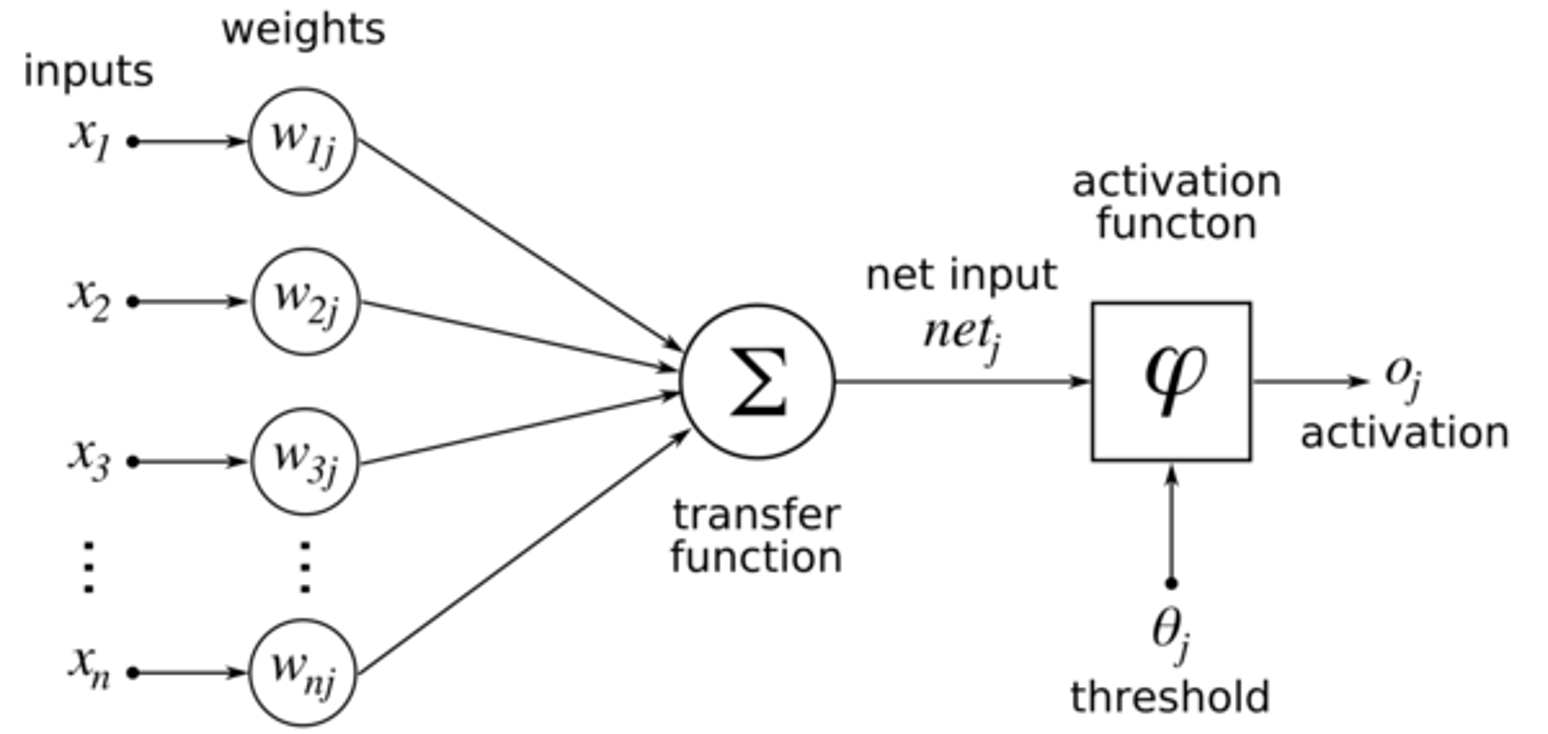
\includegraphics[width=0.7\textwidth]{./data/Diagram of Hebbian learning rule.jpg}
    \caption{Schematic Diagram of Hebbian learning rule}
    \label{fig:my_picture}
    \vspace{1pt} % Vertical space, optional
    \small{Source: \href{https://wiki.eyewire.org/Contrastive_Hebbian_learning}{Eyewire}}
\end{figure}

\begin{equation}
    w_{ij}(t + 1) = w_{ij}(t) + \alpha y_j(t)y_i
\end{equation}

Here, $w_{ij}(t+1)$ and $w_{ij}(t)$ denote the synaptic strength between neurons j and i at consecutive time points t and t + 1, respectively, while $y_i$ and $y_j$ represent their respective outputs.

The essence of Hebb's rule lies in its unsupervised learning approach, aiming to enhance synaptic connections based on the activation states of neuron pairs, thereby facilitating the modeling of elementary neural functions. This laid the groundwork for the subsequent introduction of the neuron's supervised delta learning rule, which addresses the adaptation of synaptic weights given known inputs and outputs. This method incrementally adjusts weights to align the neuron's actual output with its target output, as described below:

\begin{equation}
    w_{ij}(t + 1) = w_{ij}(t) + \alpha(d_i - y_i)x_j(t)
\end{equation}

In this formula, $\alpha$ represents the learning rate, $d_i$ the desired output, $y_i$ the actual output of neuron i, and $x_j(t)$ the input state from neuron j at time t.

Simply put, if neuron i's output exceeds the target, the weights for active connections decrease, while those for inactive connections increase. Conversely, if the actual output falls short of the target, weights for active connections are boosted, and those for inactive ones are lowered. This adaptive mechanism enables neurons to encode correct input-output mappings within their synaptic weights, thus acquiring data representation capabilities. Initially devised for individual neurons, both the Hebbian and Delta learning rules set the stage for multi-neuronal network learning algorithms, fostering the burgeoning field of neural computation and inspiring continued exploration and innovation.

\section{Delta learning rules}

Delta learning rules hinge on the principle of minimizing the discrepancy between actual network outputs and desired targets by methodically tuning the synaptic weights. The rule employs error gradient calculations to ascertain the direction and magnitude of weight adjustments. With each iteration, the network weights are modified in a direction opposite to the error gradient, progressively diminishing the error.

\begin{figure}[H]
    \centering
    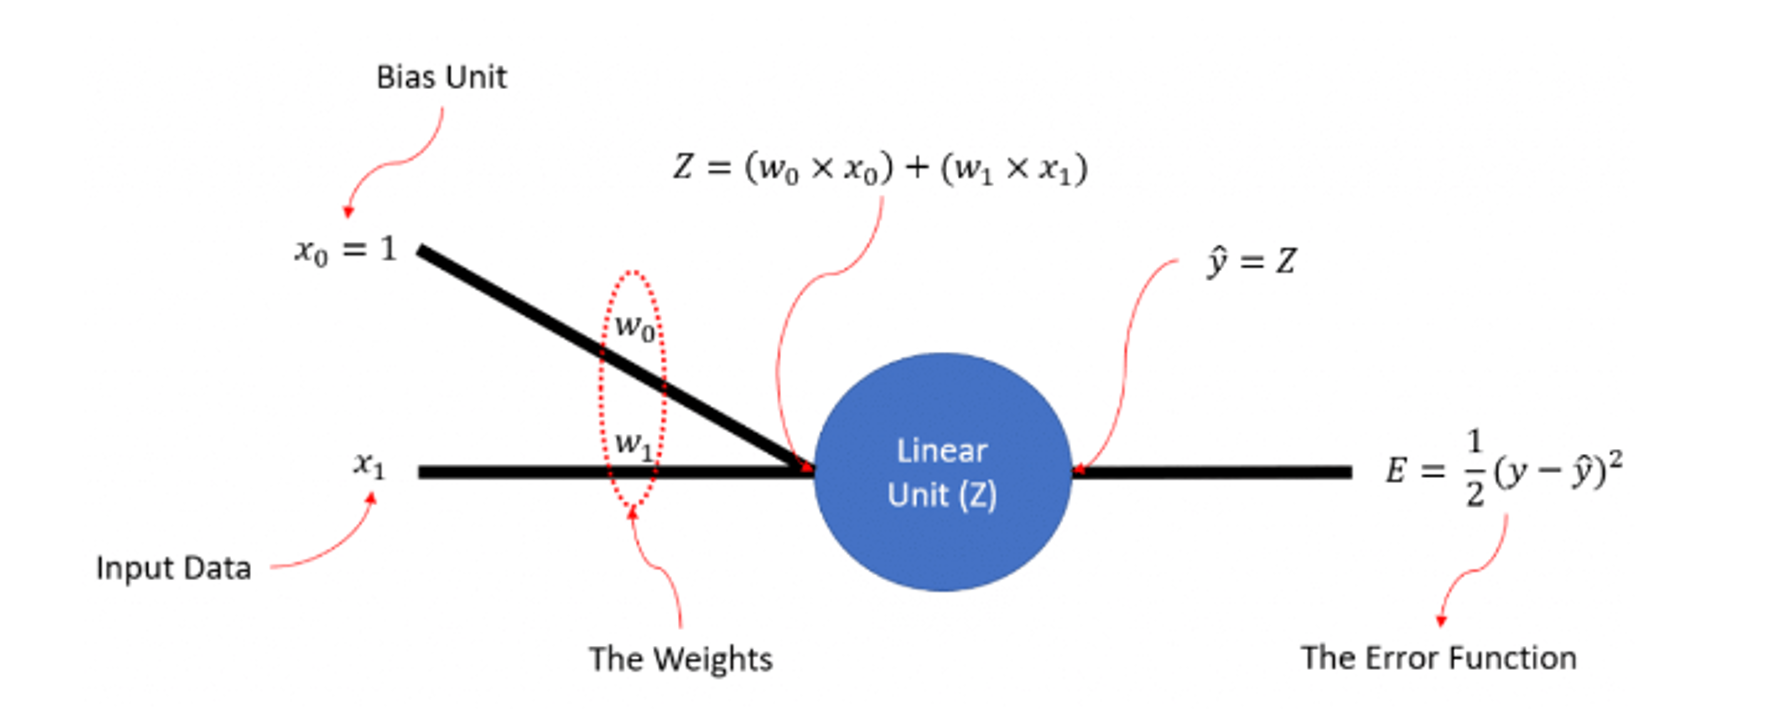
\includegraphics[width=1.0\textwidth]{./data/Diagram of Delta learning rule.jpg}
    \caption{Schematic Diagram of Delta learning rule}
    \label{fig:my_picture}
    \vspace{1pt} % Vertical space, optional
    \small{Source: \href{https://www.mldawn.com/what-is-the-delta-rule-part-1/}{Mldawn}}
\end{figure}

A prevalent form of this rule, often referred to as the delta or Widrow-Hoff rule \cite{BernardWidrow1960AdaptiveSwitchingCircuits}, is predicated on the perceptron framework. It updates weights by gauging the gap between real and intended outputs, with the magnitude of adjustment contingent upon both the input and the error signals.

The Delta, or Widrow-Hoff, learning rule, employs a straightforward algorithm for recalibrating connection weights within a neural network during its training phase. The weight adjustment formula under this rule is as follows:

\[ \Delta w_{ij} = \eta \cdot (d_j - y_j) \cdot x_i \]

Key components of this formula include:

\begin{itemize}
    \item \textbf{ $\Delta w_{ij}$:} the adjustment made to the weight from neuron \( i \) to neuron \( j \).
    \item \textbf{$\eta $:} the learning rate, dictating the scale of the weight modification.
    \item \textbf{ $d_{j}$:} the designated target output for neuron \( j \).
    \item \textbf{$y_j$:} the neuron \( j \)'s realized output.
    \item \textbf{$x_i$:} the input received by neuron \( j \) from neuron \( i \).
\end{itemize}

This mechanism calculates the weight change \( \Delta w_{ij} \) by considering the discrepancy between the target \( d_j \) and the actual output \( y_j \), factoring in the input \( x_i \) and the learning rate \( \eta \). Adjustments are applied network-wide with each training cycle.

Predominantly, Delta learning rules are instrumental in training neural networks for supervised learning tasks, including classification and regression, offering a systematic approach for networks to fine-tune weights, thereby incrementally enhancing performance and precision.

The foundational principles of both Hebbian and Delta learning rules contributed significantly to the development of the backpropagation algorithm, further enriching the landscape of neural network training methodologies.

\section{Mark I Perceptron Evolution}

In the pivotal year of 1958, F. Rosenblatt introduced the revolutionary perceptron model, marking the inception of neural network concepts into digital computation. This event signified a significant milestone in the neural networks' journey \cite{Rosenblatt1958PerceptronProbabilisticModel}. 

\begin{figure}[H]
    \centering
    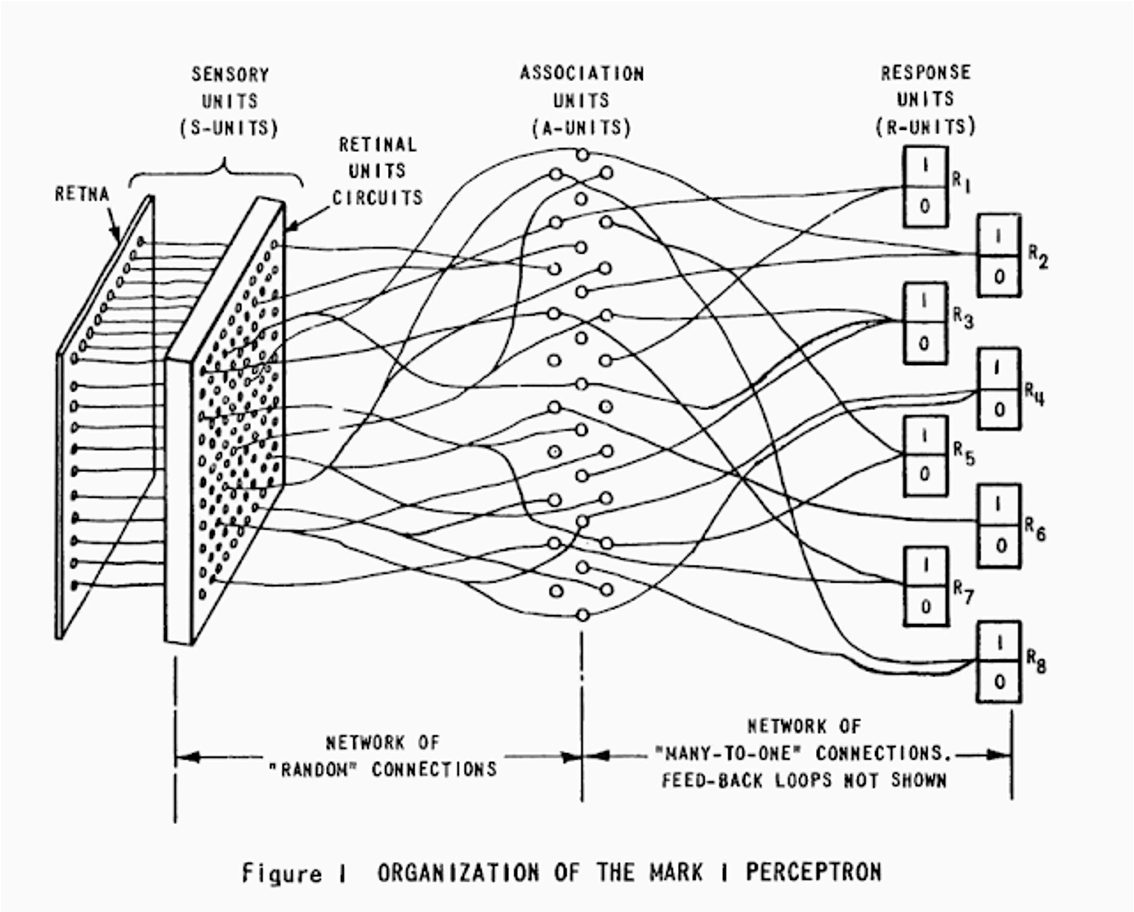
\includegraphics[width=0.7\textwidth]{./data/Architecture of Mark I perceptron.jpg}
    \caption{Architecture of Mark I perceptron}
    \label{fig:my_picture}
    \vspace{1pt} % Vertical space, optional
    \small{Source: \href{https://www.noemamag.com/blueprints-of-intelligence/}{Noema}}
\end{figure}



The perceptron, essentially a binary classifier, employs a combination of weighted inputs and a thresholding activation function to decide between two possible outcomes. It operates on the premise of:

\begin{equation}
    y = f(x) = \text{sign}(w \cdot x + b)
\end{equation}

where the input vector \( x \) and weight vector \( w \) undergo a dot product operation, with \( b \) as the bias. The \( \text{sign} \) function's role is to categorize the input as either positive or negative:

\begin{equation}
    \text{sign}(x) = 
\begin{cases}
+1, & \text{if } x \geq 0 \\
-1, & \text{if } x < 0
\end{cases}
\end{equation}

The perceptron's training algorithm iteratively adjusts its weights and bias based on classification accuracy, refining its predictive accuracy through these adjustments. Specifically, it seeks to minimize the loss function \( L(w,b) \), which is defined as the sum of errors for misclassified inputs:

\begin{equation}
L(w,b) = - \sum_{x_i \in M} y_i (w \cdot x_i + b)
\end{equation}

Gradient descent is utilized to iteratively adjust \( w \) and \( b \) in the direction that reduces \( L(w,b) \), through:

\begin{equation}
w_{\text{new}} = w_{\text{old}} + \eta y_i x_i
\end{equation}

\begin{equation}
b_{\text{new}} = b_{\text{old}} + \eta y_i
\end{equation}

with \( \eta \) denoting the learning rate. The perceptron's methodology embodies an early yet profound attempt at mimicking neuronal decision-making processes within a computational framework, named in honor of its inventor, Frank Rosenblatt.

\section{Hopfield Network Breakthrough}

The perceptron's inability to solve non-linear problems like the XOR issue, as critiqued by M. Minsky and S. Papert in "Perceptrons" (1969), paradoxically spurred advancements in neural network research. This critique indirectly prompted the development of multilayer networks and the backpropagation training method.


\begin{figure}[H]
    \centering
    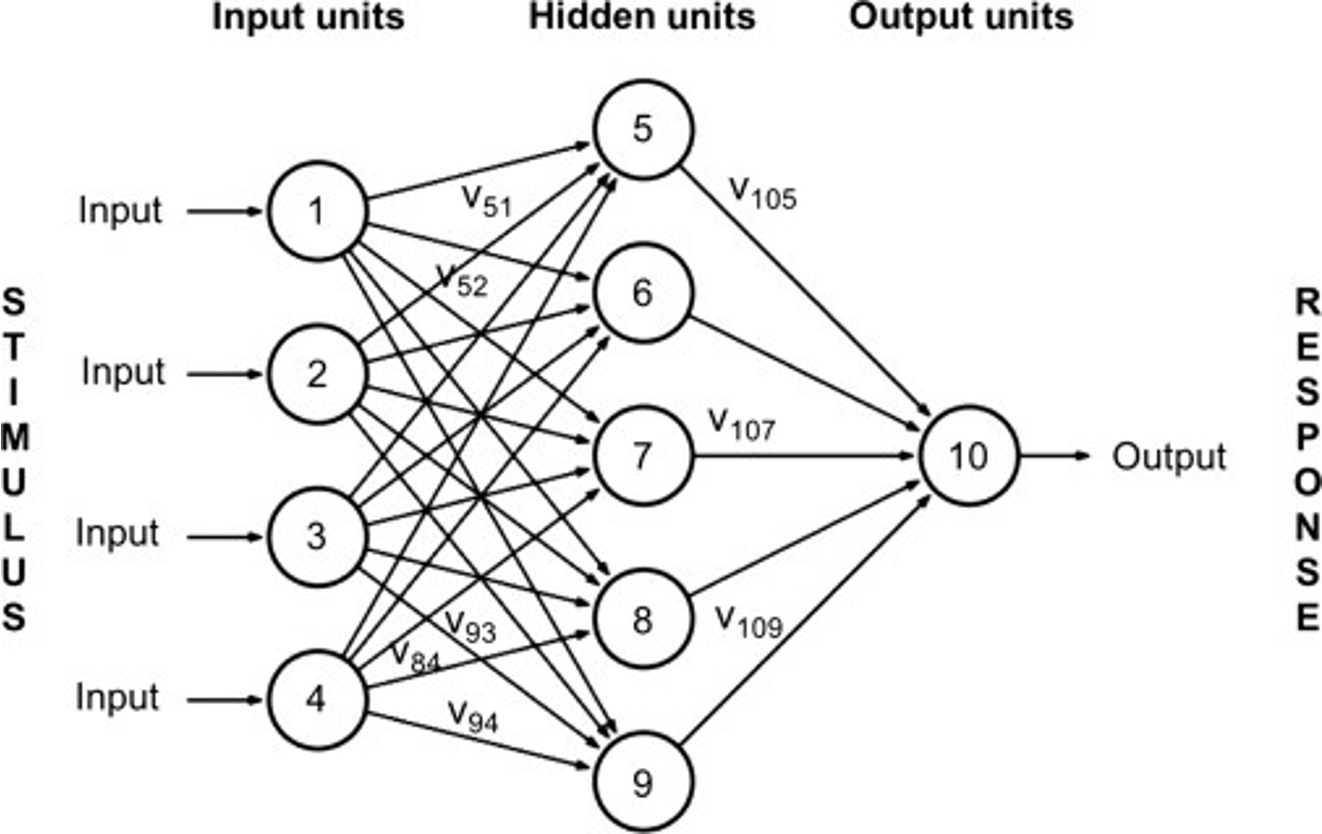
\includegraphics[width=0.7\textwidth]{./data/Architecture of Hopfield netwrok.jpg}
    \caption{Architecture of Hopfield netwrok}
    \label{fig:my_picture}
    \vspace{1pt} % Vertical space, optional
    \small{Source: \href{https://www.google.com/imgres?q=typical%20Hopfield%20Neural%20Network&imgurl=https%3A%2F%2Fars.els-cdn.com%2Fcontent%2Fimage%2F3-s2.0-B9780128184387000034-f03-02-9780128184387.jpg&imgrefurl=https%3A%2F%2Fwww.sciencedirect.com%2Ftopics%2Fcomputer-science%2Fhopfield-network&docid=_k9vh5pf2EHS1M&tbnid=EjVzB__f42R8iM&vet=12ahUKEwi07IHih_6EAxW1SEEAHX8UAAwQM3oECHQQAA..i&w=505&h=319&hcb=2&ved=2ahUKEwi07IHih_6EAxW1SEEAHX8UAAwQM3oECHQQAA}{Science Direct}}
\end{figure}


The perceptron's limitation as a linear classifier highlighted the necessity for multilayer architectures and nonlinear activation to tackle more complex, non-linear problems. A significant stride in this direction was J.J. Hopfield's 1982 innovation of a network model capable of associative memory, revolutionizing the use of neural networks for optimization challenges, such as the Travelling Salesman Problem \cite{JJHopfield1982NeuralNetworksPhysical}.

The Hopfield network is notable for its utilization of feedback loops, establishing an energy-minimizing model that was a novel approach for optimization in computational tasks. This framework not only advanced the theoretical understanding of neural networks but also laid foundational principles for the development of sophisticated, pattern-recognizing neural systems.

Hopfield networks introduced a dynamic memory model, differing significantly from the perceptron's static memory approach. This capability for associative memory—recalling patterns based on partial inputs—represented a leap forward in computational memory systems.

The contributions of Hopfield's work catalyzed a renewed interest in neural network research, setting the stage for further innovations such as the Boltzmann machine by G.E. Hinton and others in 1983. This progression built upon Hopfield's model, expanding the capabilities of neural networks to address a broader spectrum of computational problems.


\chapter{Hodgkin-Huxley Model}

\section{Introduction}

The Hodgkin-Huxley model, proposed by Sir Alan Hodgkin and Sir Andrew Huxley in 1952, revolutionized the field of neuroscience by providing a quantitative understanding of the generation and propagation of action potentials in neurons. This mathematical framework emerged from a decade-long collaboration between Hodgkin and Huxley, culminating in the publication of their landmark papers in the Journal of Physiology.

\subsubsection{Historical Background}

The Hodgkin-Huxley theory emerged as a result of a remarkable collaboration between Hodgkin and Huxley from the late 1930s to the early 1950s. Their work was informed by several key experimental findings. Cole and Curtis demonstrated that the action potential is associated with a significant increase in membrane conductance, laying the groundwork for understanding neuronal excitability\cite{Cole1939}. Subsequently, Hodgkin and Huxley performed the first intracellular recording of an action potential, revealing that the membrane potential during an action potential exceeds zero mV, thereby challenging existing hypotheses\cite{Hodgkin1939}. This experimental breakthrough was complemented by the theoretical insights of Hodgkin and Katz, who explained the overshooting action potential by elucidating the role of sodium permeability\cite{Hodgkin1949}. Additionally, Hodgkin, Huxley, and Katz developed a voltage-clamp circuit, following the pioneering work of Cole and Marmont, enabling precise measurement of ionic currents in squid axons\cite{Hausser2000}.

\section{Biological Basis of Neuronal Excitability}

Neuronal excitability, the ability of neurons to generate and transmit electrical signals, is fundamental to their function in the nervous system. This excitability arises from the intricate interplay of ion channels and the dynamic changes in membrane potential they produce.

\subsection{Resting Membrane Potential}

The resting membrane potential of a neuron, typically ranging from -60 mV to -70 mV, is maintained by the selective permeability of the cell membrane to different ions. This selective permeability is primarily mediated by resting ion channels, particularly those permeable to potassium ions. At rest, these channels allow a small efflux of K+ ions, establishing the negative charge within the cell compared to the extracellular space.

\begin{figure}[htbp]
    \centering
    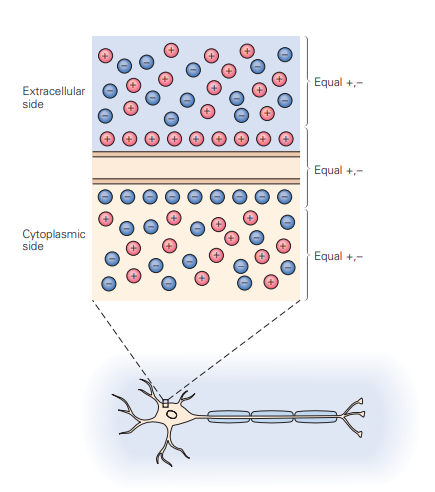
\includegraphics[width=0.6\textwidth]{./data/resting_membrane_potential.png}
    \caption{Resting membrane potential (Source: Principles of Neural Science\cite{principles_of_neural_science})}
    \label{fig:resting_membrane_potential}
\end{figure}

\subsection{Generation of Action Potentials}

Action potentials, the transient electrical signals responsible for rapid communication within the nervous system, are generated when the membrane potential depolarizes beyond a certain threshold. This depolarization is initiated by the opening of voltage-gated sodium channels in response to a stimulus. As Na+ ions rush into the cell, the membrane potential becomes more positive, reaching around +40 mV.

\subsection{Propagation of Action Potentials}

Once initiated, the action potential propagates along the axon of the neuron. This propagation occurs through a self-regenerating process where the depolarization of one region of the membrane triggers the opening of voltage-gated sodium channels in the adjacent region, leading to further depolarization. This continues along the length of the axon, allowing the action potential to travel rapidly towards the synapse.

\subsection{Repolarization and Hyperpolarization}

Following depolarization, the membrane potential undergoes repolarization, returning to its resting state. This repolarization is driven by the opening of voltage-gated potassium channels, allowing K+ ions to exit the cell, while voltage-gated sodium channels undergo inactivation. In some cases, repolarization may overshoot, leading to hyperpolarization, before eventually returning to the resting membrane potential\cite{principles_of_neural_science}.

\section{Formulation of the Hodgkin-Huxley Model}

The Hodgkin-Huxley model provides a quantitative description of membrane currents and their role in nerve conduction and excitation. Central to this model is the representation of the neuronal membrane as an electrical circuit, which captures the dynamics of ion flow across the membrane during the generation and propagation of action potentials.

\begin{figure}[htbp]
    \centering
    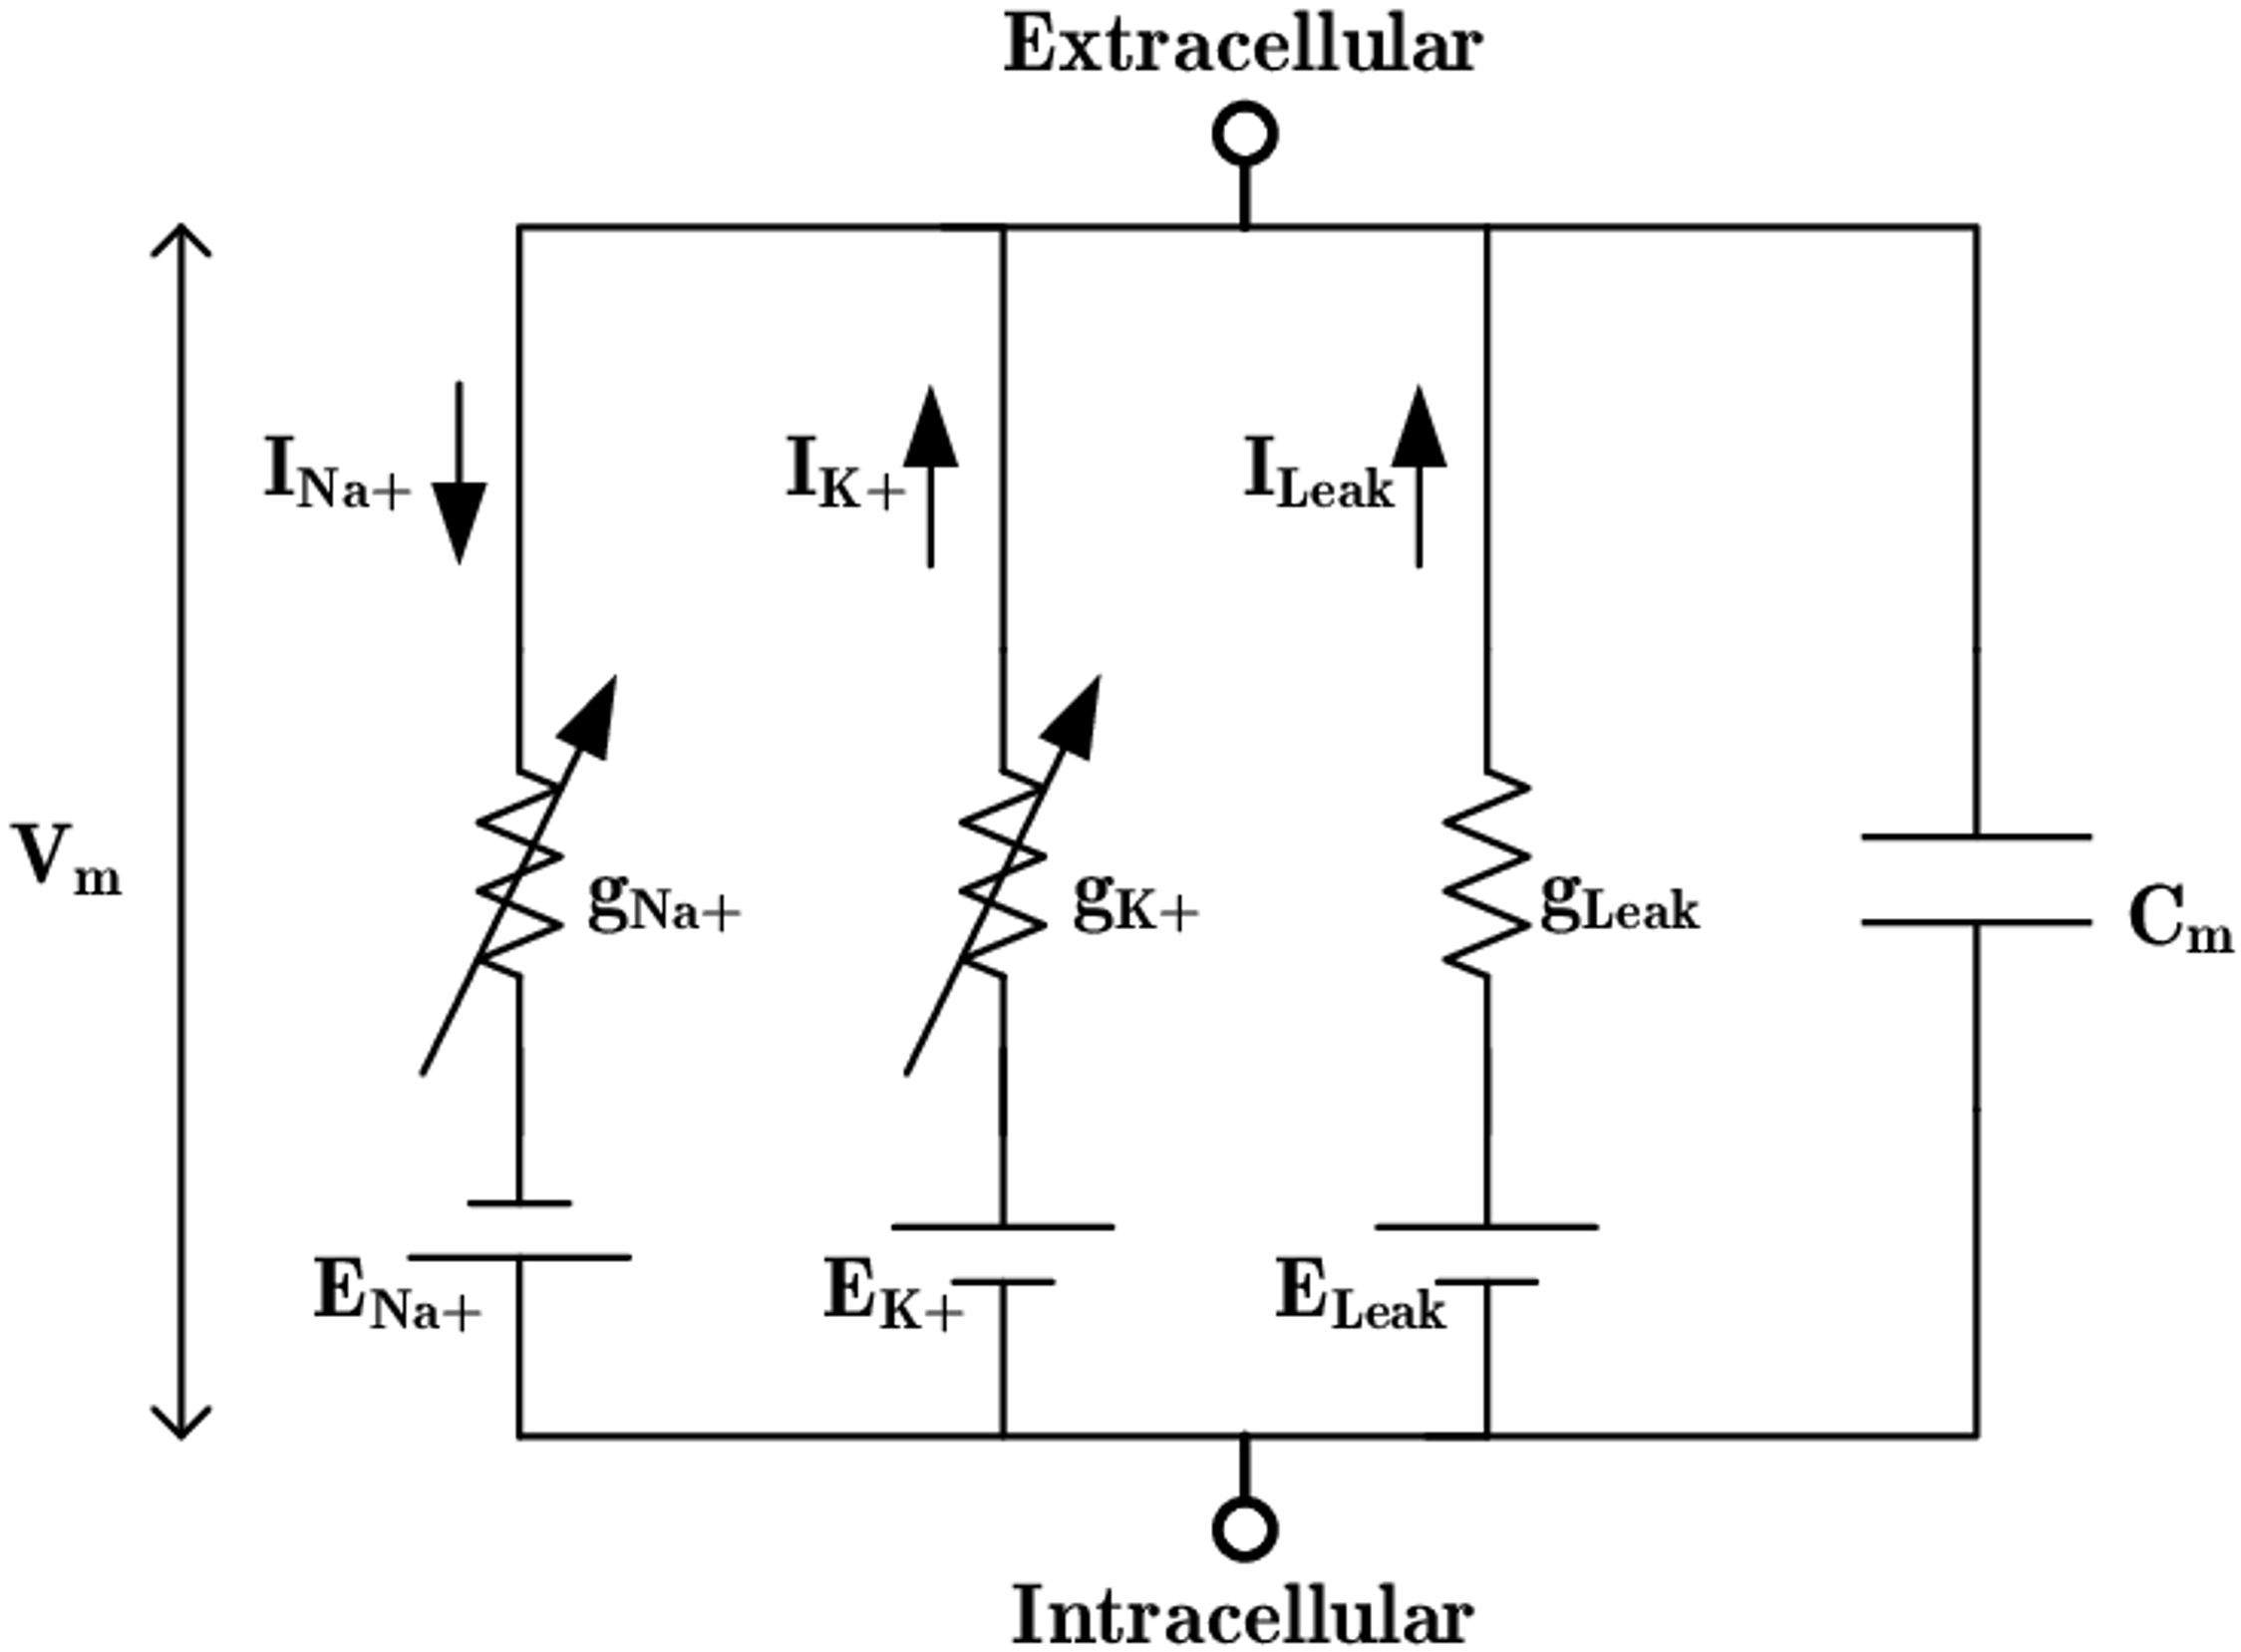
\includegraphics[width=0.6\textwidth]{./data/electrical_circuit_representing membrane.png}
    \caption{Electrical circuit representing membrane. (Source: A quantitative description of membrane current and its application to conduction and excitation in nerve\cite{Hodgkin1952})}
    \label{fig:electrical_circuit_representing membrane.}
\end{figure}

\subsection{Electrical Circuit Representation}

In the Hodgkin-Huxley model, the neuronal membrane is represented as an electrical circuit composed of several components.

Membrane Capacitance (C): The lipid bilayer of the neuronal membrane acts as a capacitor, storing charge and contributing to the membrane's ability to maintain a voltage gradient.

Ion Channels: Voltage-gated ion channels, including sodium (Na+), potassium (K+), and leak channels, are represented as resistors in the circuit. These channels control the flow of ions across the membrane in response to changes in membrane potential.

Battery (Em): The battery in the circuit represents the resting membrane potential, which is typically around -60 to -70 mV in neurons. It serves as the reference voltage against which changes in membrane potential are measured.

\subsection{The Hodgkin-Huxley Equation}

The Hodgkin-Huxley model provides a quantitative description of membrane current and its application to conduction and excitation in nerve cells. It represents the dynamic interplay of ion channels and membrane capacitance in generating and propagating action potentials.

The model is formulated based on the principles of electrical circuits. The total current in the neuron can be expressed as the sum of the individual ion currents and the capacitive current:
\[
I_{\text{Total}} = I_{\text{Na}} + I_{\text{K}} + I_{\text{leak}} + I_{\text{C}}
\]

Using the relationship between charge ($Q$), capacitance ($C$), and potential difference ($V$):
\[
C = \frac{Q}{V}
\]

We can express the capacitive current ($I_C$) as the rate of change of charge with respect to time:
\[
C \frac{dV}{dt} = I_{\text{Total}} - I_{\text{Na}} - I_{\text{K}} - I_{\text{leak}}
\]

Applying Ohm's law ($I = \frac{V}{R}$), where $R$ is the resistance, to each ion current:
\[
I = \frac{1}{R} \times V
\]

We can modify this to incorporate the reversal potential ($E$):
\[
I = \frac{1}{R} \times (V - E)
\]

Substituting these into the equation for the capacitive current:
\[
C \frac{dV}{dt} = I_{\text{Total}} - \frac{1}{R_{\text{Na}}} \times (V_m - E_{\text{Na}}) - \frac{1}{R_{\text{K}}} \times (V_m - E_{\text{K}}) - \frac{1}{R_{\text{leak}}} \times (V_m - E_{\text{leak}})
\]

Where $V_m$ represents the membrane potential, and $E_{\text{Na}}$, $E_{\text{K}}$, and $E_{\text{leak}}$ represent the equilibrium potentials for sodium, potassium, and leak currents respectively.

Expanding the equation using the Hodgkin-Huxley model for the conductance of each ion ($g$) and the gating variables ($m$, $h$, $n$):
\begin{align*}
C \frac{dV}{dt} & = I_{\text{Total}} - g_{\text{Na}} m^3 h (V_m - E_{\text{Na}}) \\
                 & \quad - g_{\text{K}} n^4 (V_m - E_{\text{K}}) - g_{\text{leak}} (V_m - E_{\text{leak}})
\end{align*}

Where
\[
\frac{dm}{dt} = -\frac{(m - m_{\infty}(V))}{\tau_m(V)}, \quad \frac{dh}{dt} = -\frac{(h - h_{\infty}(V))}{\tau_h(V)}, \quad \frac{dn}{dt} = -\frac{(n - n_{\infty}(V))}{\tau_n(V)}
\]
represent the gating variable dynamics.

\begin{itemize}
  \item The equation $\frac{dm}{dt} = -\frac{(m - m_{\infty}(V))}{\tau_m(V)}$ represents the dynamics of the gating variable $m$. 
  \begin{itemize}
    \item $m$ represents the activation gating variable for sodium channels.
    \item $m_{\infty}(V)$ is the steady-state value of $m$ at membrane potential $V$, which describes the fraction of sodium channels that are open.
    \item $\tau_m(V)$ is the time constant associated with the activation gating variable $m$, which determines how quickly $m$ changes with respect to time.
  \end{itemize}
  
  \item Similarly, the equation $\frac{dh}{dt} = -\frac{(h - h_{\infty}(V))}{\tau_h(V)}$ represents the dynamics of the gating variable $h$.
  \begin{itemize}
    \item $h$ represents the inactivation gating variable for sodium channels.
    \item $h_{\infty}(V)$ is the steady-state value of $h$ at membrane potential $V$, which describes the fraction of sodium channels that are inactivated.
    \item $\tau_h(V)$ is the time constant associated with the inactivation gating variable $h$, determining how quickly $h$ changes over time.
  \end{itemize}
  
  \item Finally, the equation $\frac{dn}{dt} = -\frac{(n - n_{\infty}(V))}{\tau_n(V)}$ represents the dynamics of the gating variable $n$.
  \begin{itemize}
    \item $n$ represents the activation gating variable for potassium channels.
    \item $n_{\infty}(V)$ is the steady-state value of $n$ at membrane potential $V$, indicating the fraction of potassium channels that are open.
    \item $\tau_n(V)$ is the time constant associated with the activation gating variable $n$, governing how quickly $n$ changes with time.
  \end{itemize}
\end{itemize}

These equations describe how the gating variables $m$, $h$, and $n$ change over time in response to changes in membrane potential $V$. They play a crucial role in determining the conductance of sodium and potassium channels, which, in turn, influences the generation and propagation of action potentials in neurons\cite{Hodgkin1952}.


\section{Python Simulation}

This section presents the results of the simulation using the Hodgkin-Huxley model for different applied external currents. The simulation was conducted to understand the behavior of the neuron in response to varying input stimuli and to validate the model against known physiological phenomena.

\subsubsection{Simulation Results}
The Hodgkin-Huxley model explains how the dynamics of ion channels (Na+, K+ etc) contribute to the generation of an Action Potential in a neuron.
An Action Potential is a sharp voltage spike elicited by stimulating a neuron with a current
that exceeds a certain threshold value. The current amplitude is increased gradually, at a
threshold amplitude, the voltage response does not increase proportionally.
It shows a sharp, disproportionate increase.
Once the membrane voltage reaches a threshold value, it increases further rapidly to maximum value and drops again rapidly to a value that is less than resting value, before returning
to the baseline value after a delay.


\begin{itemize}
  \item For input currents ranging from 0µA to 0.02235µA, no action potentials were observed.
\end{itemize}

\begin{itemize}
  \item A sudden onset of action potentials occurred when the input current was increased from 0.02235µA to 0.02236µA. However, these action potentials were not periodic.
\end{itemize}

\begin{itemize}
  \item Periodic action potentials were observed when the input current was further increased from 0.0622µA to 0.06223µA.
\end{itemize}

\begin{itemize}
  \item For input currents ranging from 0.06223µA to 0.450µA, periodic action potentials were observed.
\end{itemize}

\begin{itemize}
  \item Action potentials ceased when the input current was increased beyond 0.450µA.
\end{itemize}

\begin{figure}[H]
    \centering
    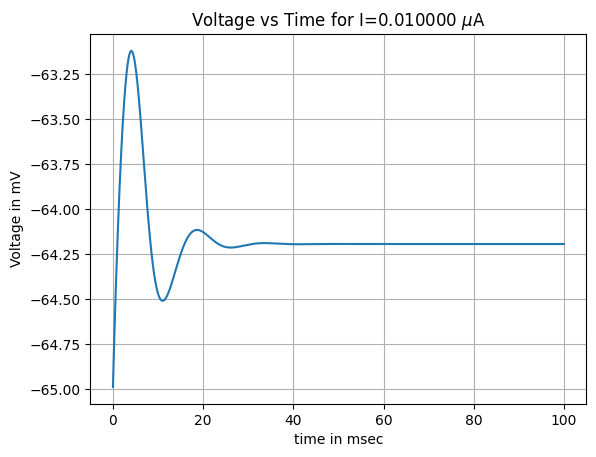
\includegraphics[width=0.6\textwidth]{./data/voltage_time_0_01uA.png}
    \caption{Plot of Voltage vs Time for I=0.01µA}
    \label{fig:voltage_time_0_01uA}
\end{figure}

\begin{figure}[H]
    \centering
    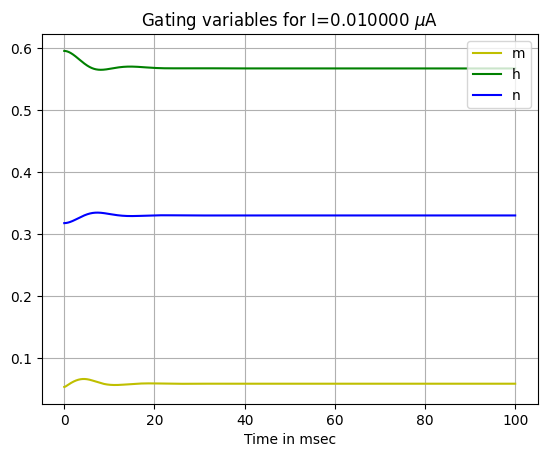
\includegraphics[width=0.6\textwidth]{./data/gating_variables_0_01uA.png}
    \caption{Plot of gating variables for I=0.01µA}
    \label{fig:gating_variables_0_01uA}
\end{figure}

\begin{figure}[H]
    \centering
    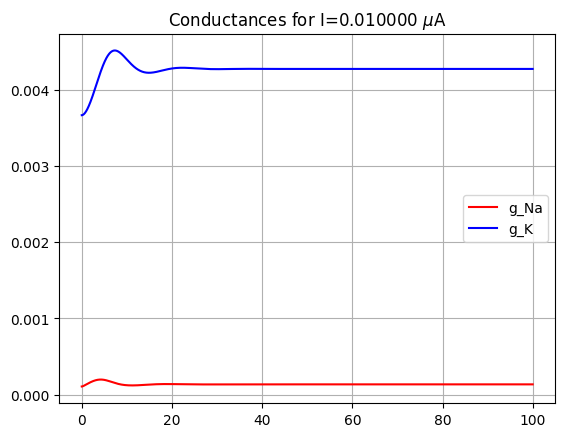
\includegraphics[width=0.6\textwidth]{./data/conductances_0_01uA.png}
    \caption{Plot of conductances for I=0.01µA}
    \label{fig:conductances_0_01uA}
\end{figure}



\begin{figure}[H]
    \centering
    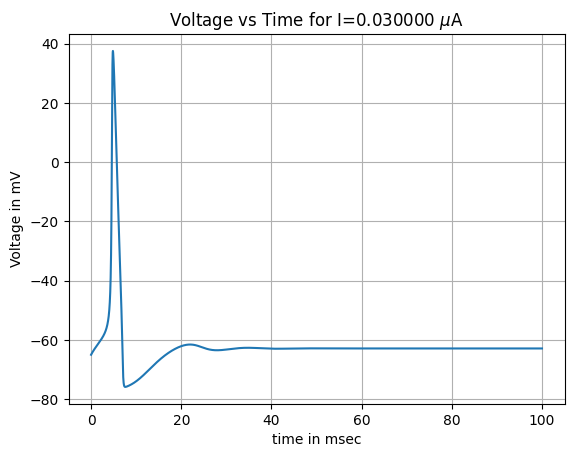
\includegraphics[width=0.6\textwidth]{./data/voltage_time_0_03uA.png}
    \caption{Plot of Voltage vs Time for I=0.03µA}
    \label{fig:voltage_time_0_03uA}
\end{figure}

\begin{figure}[H]
    \centering
    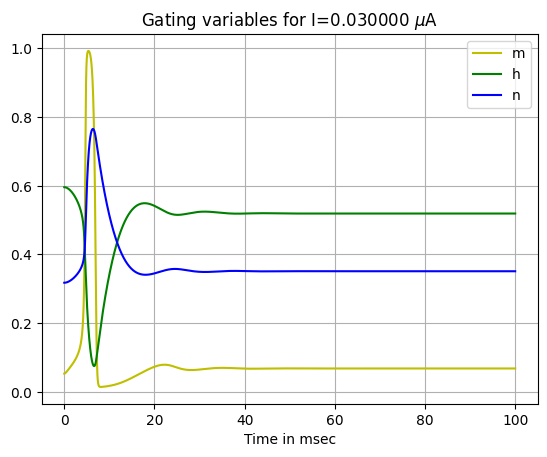
\includegraphics[width=0.6\textwidth]{./data/gating_variables_0_03uA.png}
    \caption{Plot of gating variables for I=0.03µA}
    \label{fig:gating_variables_0_03uA}
\end{figure}

\begin{figure}[H]
    \centering
    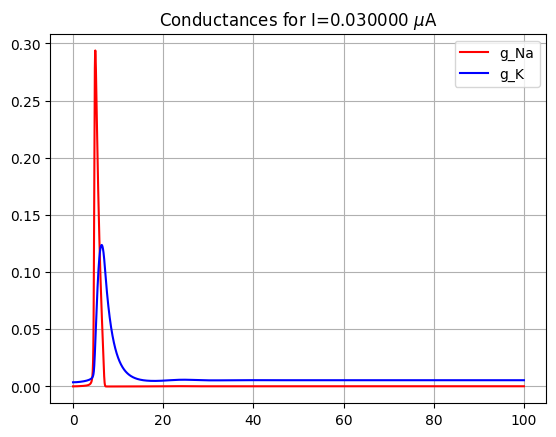
\includegraphics[width=0.6\textwidth]{./data/conductances_0_03uA.png}
    \caption{Plot of conductances for I=0.03µA}
    \label{fig:conductances_0_03uA}
\end{figure}



\begin{figure}[H]
    \centering
    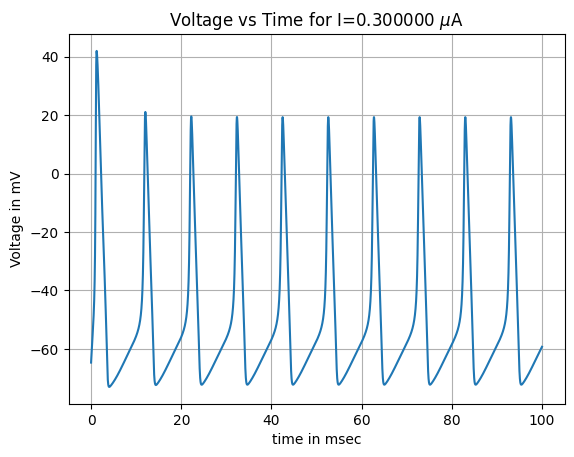
\includegraphics[width=0.6\textwidth]{./data/voltage_time_0_3uA.png}
    \caption{Plot of Voltage vs Time for I=0.3µA}
    \label{fig:voltage_time_0_3uA}
\end{figure}

\begin{figure}[H]
    \centering
    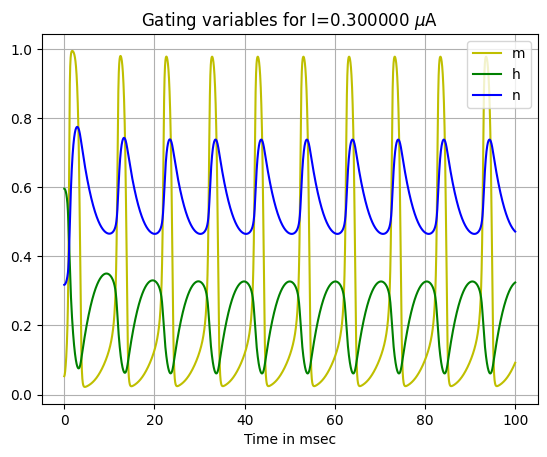
\includegraphics[width=0.6\textwidth]{./data/gating_variables_0_3uA.png}
    \caption{Plot of gating variables for I=0.3µA}
    \label{fig:gating_variables_0_3uA}
\end{figure}

\begin{figure}[H]
    \centering
    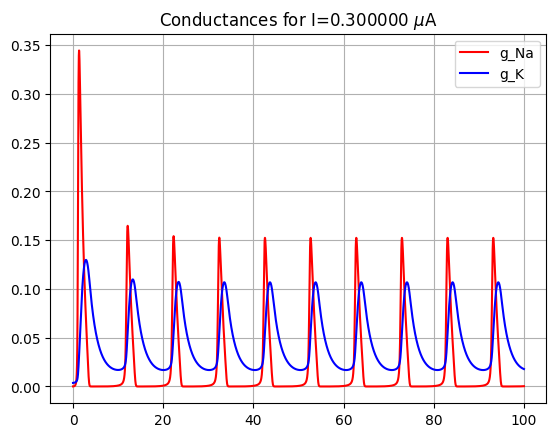
\includegraphics[width=0.6\textwidth]{./data/conductances_0_3uA.png}
    \caption{Plot of conductances for I=0.3µA}
    \label{fig:conductances_0_3uA}
\end{figure}

\begin{figure}[H]
    \centering
    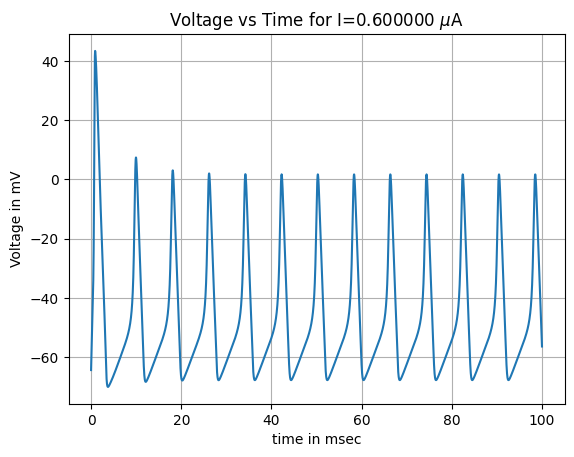
\includegraphics[width=0.6\textwidth]{./data/voltage_time_0_6uA.png}
    \caption{Plot of Voltage vs Time for I=0.6µA}
    \label{fig:voltage_time_0_6uA}
\end{figure}

\begin{figure}[H]
    \centering
    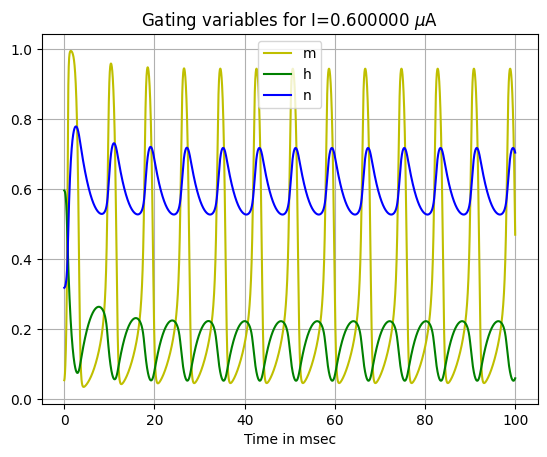
\includegraphics[width=0.6\textwidth]{./data/gating_variables_0_6uA.png}
    \caption{Plot of gating variables for I=0.6µA}
    \label{fig:gating_variables_0_6uA}
\end{figure}

\begin{figure}[H]
    \centering
    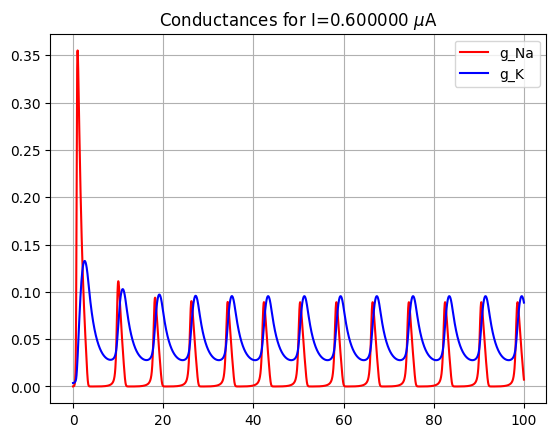
\includegraphics[width=0.6\textwidth]{./data/conductances_0_6uA.png}
    \caption{Plot of conductances for I=0.6µA}
    \label{fig:conductances_0_6uA}
\end{figure}


\chapter{Dynamics Of Neuron}

\section{Elements of Neuronal Systems}

Various types of neurons can be distinguished by the shape of their cell bodies and extensions. However, the network of neurons in the cortex is much more complex than what can be captured in a single picture. In fact, the cortex contains over \(10^{4}\) cell bodies and several kilometers of \textit{wires} per cubic millimeter, densely packed into a complex network that varies across different areas of the brain \cite{ref1}. Despite the differences in wiring patterns, all areas of the brain rely on neurons of different shapes and sizes as their building blocks. An example of such a neuronal network is depicted in Fig. 5.1, based on the early 20th century work of neuroscience pioneer Ramón y Cajal \cite{ref1}.

% Your figure code with the H specifier to force placement here
\begin{figure}[H]
\centering % Centers the figure
\fbox{% Adds a border to the figure
  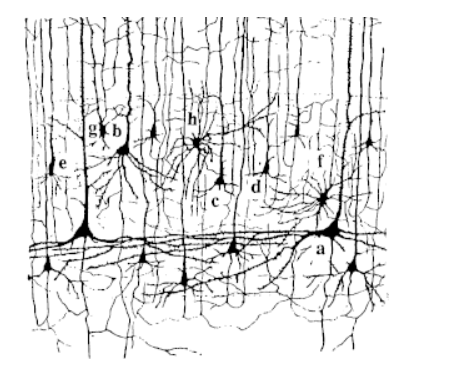
\includegraphics[width=0.8\textwidth]{./data/drawing.png} % Adjusts the size
}
\caption{A drawing of Ramón y Cajal showing a few neurons in the mammalian cortex \cite{ref2}} 
\end{figure}

The illustration reveals various neurons with distinct cell bodies and elongated projections, providing a snapshot of the densely woven neuronal networks in the cortex. In reality, the cortex’s neuronal networks are even more elaborate, with over 10,000 neuron cell bodies and extensive wiring in just one cubic millimeter. However, neurons are not the sole constituents of the cortex. It also comprises a multitude of glial cells, which play a supportive role in the brain’s energy management and structural integrity \cite{ref2}. 

When considering the physiology of neurons, it is important to note that their internal potential at rest is typically negative in comparison to their surroundings, often around -70mV. This negative resting potential is established by the combined action of various gating mechanisms, ion pumps, and ion channels present in the cell membrane \cite{ref3}. However, when the neuron's resting potential is perturbed beyond a certain level, such as due to input from other neurons, the ion channels in the membrane open and close in a coordinated manner to allow mainly ionic sodium and potassium (but also calcium and chloride) to pass through the membrane, resulting in a rapid and sharp change in potential. This sudden change generates a stereotyped pulse, or action potential, which travels along the axon of the neuron in an all-or-nothing manner, meaning that it is either fired with full amplitude or not fired at all.

The Hodgkin and Huxley model, developed over 50 years ago, provides a detailed description of a single neuron as a modified electrical circuit that transports electrical signals \cite{ref4}. This model explains how a single cell can regulate flows of ions through its cell membrane to rapidly depolarize and re-polarize itself, allowing for the generation of action potentials that become outputs to other neurons. In the human brain, which consists of approximately \(10^{11}\) neurons and \(10^{15}\) connections, neurons work as summing devices that sum up all their inputs, and depending on whether this sum reaches a certain threshold, respond by generating action potentials that become outputs to other neurons \cite{ref5}. These inputs may be either excitatory or inhibitory, resulting in an increase or decrease in the probability of the receiver neuron firing a response signal.

The brain processes information mainly by transmitting electric signals (action potentials) between millions of neurons across nerve fibers, with most modeling approaches considering only a subset of these. The fundamental questions in understanding the brain deal with how the activity of high numbers of interconnected neurons gives rise to a global activity pattern that is related to the function of the brain.


\begin{figure}[H]
    \centering % Centers the figure
    \fbox{% Adds a border to the figure
      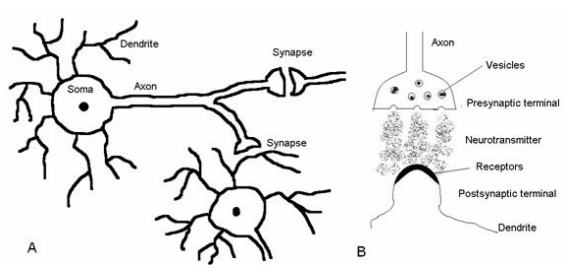
\includegraphics[width=0.8\textwidth]{./data/neuron.png} % Adjusts the size
    }
    \caption[A: A simple sketch of two neurons connected by a chemical synapse; B: A sketch of a chemical synapse]{\textbf{A:} A simple sketch of two neurons connected by a chemical synapse; \\ \textbf{B:} A sketch of a chemical synapse} 
\end{figure}
    
The brain adapts to environmental events and changes at three different time scales  \cite{ref6}. At the longest time scale, genetic adaptation results in a hard-wired connectivity of the neural network. At an intermediate time scale, the central nervous system adapts through numerous plastic mechanisms, forming assemblies of highly interacting and functionally associated neurons. Finally, at the shortest time scale, highly temporal changes in the neural activity are associated with the short-term states of the brain, which are closely related to cognitive processes \cite{ref7}.


\section{Neuron dynamics}
The human nervous system is composed of billions of individual nerve cells called neurons. Each neuron has a distinct structure that can be divided into segments such as the cell body, axon, and dendrites. The cell body contains the nucleus and other organelles that are essential for the neuron's proper functioning. The axon is a long, slender extension that carries electrical signals away from the cell body to other neurons or muscle cells. The dendrites are shorter, branched extensions that receive signals from other neurons and transmit them to the cell body. 

These different segments of the neuron work together to propagate action potentials, which are brief electrical impulses that allow neurons to communicate with one another. The interaction between the segments can be described as autonomous nonlinear systems, meaning that they operate independently and can exhibit complex, nonlinear behavior \cite{ref7}. These systems are crucial to the proper functioning of the nervous system, allowing us to perceive, process, and respond to the world around us.
\subsection{The Fitzhugh–Nagumo model}
The Fitzhugh-Nagumo model is a simplified mathematical representation of the neural dynamics of a neuron. It is essentially a third-order limit-cycle oscillator, which is characterized by the presence of two variables: the membrane potential V and the activation parameter n. The model exhibits different types of behavior depending on the control parameter a. Specifically, the system can display either stable fixed-point behavior or limit cycles. This model can shows table fixed-point behavior (Figs. 5.3(a) and (d)) or limit cycles (Figs. 5.3(c) and 3(d)), depending on the value of the control parameter. 


\begin{figure}[H]
    \centering % Centers the figure
    \fbox{% Adds a border to the figure
      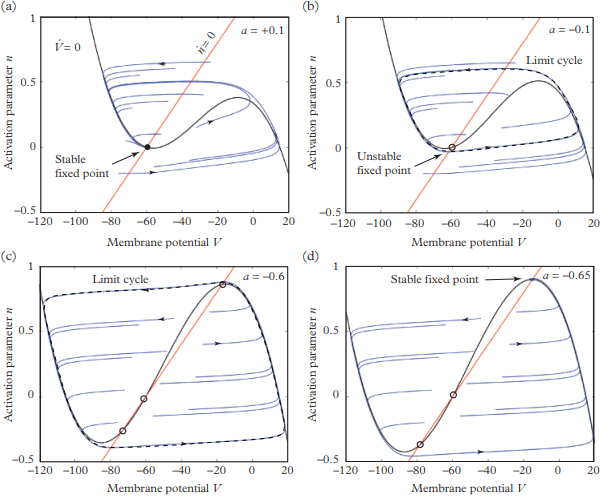
\includegraphics[width=0.8\textwidth]{./data/Fitzmodel.png} % Adjusts the size
    }
    \caption{Examples of the Fitzhugh–Nagumo model. The graph shows the membrane potential V on the horizontal axis and the activation parameter n on the vertical axis. The nullclines are plotted for n and V for I = 0. For a = +0.1, there is a stable fixed point in (a), while in (b) and (c) there are limit cycles representing neural spiking. In (d) for a = -0.67, the system converts back to a stable fixed point. \cite{ref8}} 
\end{figure}
    
When the stimulus is weak, the system is at a stable fixed point. In other words, it remains in a steady state, with the membrane potential and activation parameter both maintaining constant values. However, as the strength of the stimulus increases, the system undergoes a transition from resting potential to spiking. This means that the neuron starts to generate action potentials, which are brief but large electrical impulses that propagate along its axon and enable it to communicate with other neurons. The frequency and amplitude of these spikes can vary depending on the strength and duration of the stimulus\cite{ref8}. Overall, the Fitzhugh-Nagumo model provides a useful framework for understanding the basic mechanisms of neural activity and how they can be modulated by external inputs.
    
\subsection{The NaK model}
The NaK model is a sophisticated mathematical representation that illuminates the intricacies of two-dimensional phase planes. Its intriguing dynamics are contingent upon the bias current I, which can result in complex patterns of bistability and bifurcations. As a result, this model is highly useful for delving deeper into the parameter space and comprehending the diverse range of behaviors that it can exhibit. One of the interesting features of the NaK model is its ability to display bistability, which is an important aspect of neurodynamics. 

When a transient pulse is applied to the system, it can cause the system to cross the separatrix into the region where the dynamics relax onto the limit cycle. Once the system is on the limit cycle, it persists in a continuous oscillation. This type of behavior is characteristic of many biological systems, and the NaK model is a useful tool for studying and understanding these dynamics \cite{ref9}. The NaK model can display bifurcations as well as bistability. It allows a neuron to spike continuously even after the stimulus has been removed. 

When a short-lived pulse is introduced and then promptly withdrawn, it can elicit a response from the system that leads it to cross the separatrix and enter a state of sustained oscillation along a limit cycle \cite{ref10}. This phenomenon is illustrated in Fig. 5.4, and is observed in the NaK model when exposed to a current pulse of brief duration.


\begin{figure}[H]
    \centering % Centers the figure
    \fbox{% Adds a border to the figure
      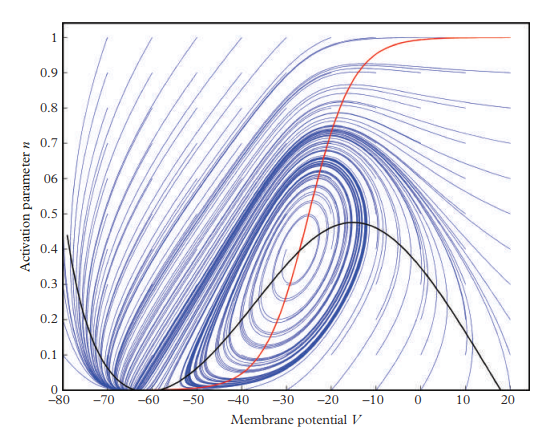
\includegraphics[width=0.8\textwidth]{./data/nak1.png} % Adjusts the size
    }
    \caption{Streamlines for the NaK model, show bistability\cite{ref9}} 
\end{figure}
    
    
Fig. 5.5 displays the phase diagram of the NaK model, which illustrates the situation where the stable node and the saddle point merge into a single saddle point. At this point, the limit cycle becomes a homoclinic orbit with an infinite period. This type of bifurcation is referred to as a saddle bifurcation, which can also be called a fold or a tangent bifurcation. In the NaK model, the harmonic orbit is connected to the saddle point.
    

\begin{figure}[H]
    \centering % Centers the figure
    \fbox{% Adds a border to the figure
      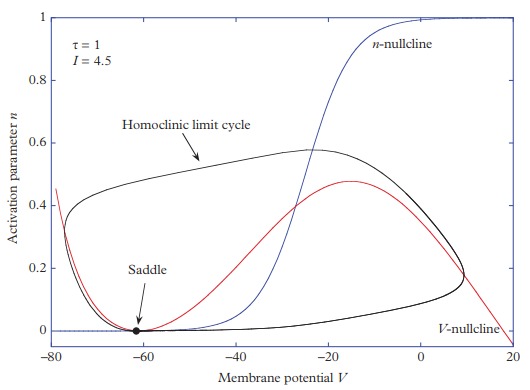
\includegraphics[width=0.8\textwidth]{./data/fig5.png} % Adjusts the size
    }
    \caption{A homoclinic orbit in the NaK model connected to the saddle point.\cite{ref9}} 
\end{figure}
    
Finally, the membrane potential for a trajectory close to the homoclinic orbit is demonstrated in Fig. 5.6. During the rapid traversal of the orbit, the membrane potential undergoes a quick change, and this is followed by a slow approach to the saddle point. This slow approach leads to a characteristic spiking appearance of the membrane potential. The spiking pattern is a result of the slow approach to the saddle, which causes the membrane potential to oscillate back and forth \cite{ref10}. These oscillations are responsible for the spiking appearance of the membrane potential.

\begin{figure}[H]
    \centering % Centers the figure
    \fbox{% Adds a border to the figure
      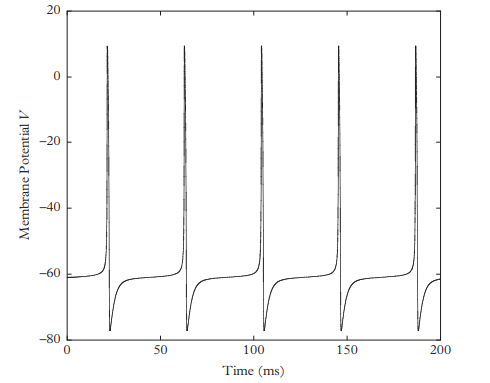
\includegraphics[width=0.8\textwidth]{./data/Fig6.png} % Adjusts the size
    }
    \caption{Membrane potential for an orbit near the homoclinic orbit as a time function.\cite{ref10}} 
\end{figure}



\chapter{Applications}
Biological neural network modeling is pushing the technological frontier in every field by simulating biological neural networks, solving real-world challenges, and improving the quality of human life. These applications demonstrate the power of interdisciplinary collaboration, bringing together biology, computer science, engineering and medicine to advance the future of medical technology and technology.

\begin{itemize}
    \item \textbf{ Brain-Computer Interface (BMI):} Brain-computer interface technology allows the human brain to interact directly with external devices, which has significant potential in providing assistive tools and restoring limb movement to paraplegic patients. Through the application of biological neural network models, researchers can better understand how brain signals map to body movements and how these signals can be interpreted to control external devices. These models also help improve algorithms to decode and translate brain activity into mechanical movements or electrical signals, enhancing the accuracy and responsiveness of brain-computer interfaces.
    \item \textbf{AI:} Biological neural networks provide artificial intelligence with a framework that mimics complex brain processing functions, particularly in the areas of vision and language processing. Deep learning, a biologically inspired algorithm, has led to breakthroughs in image recognition, speech-to-text conversion, and machine translation. Advances in these technologies, due in part to the understanding and simulation of how biological neural networks work, are changing the way we interact with technology and are finding applications in areas such as medicine, self-driving vehicles and smart homes.
    \item \textbf{Cognitive and Behavioral Research:} Biological neural network modeling helps scientists understand how cognitive processes are encoded in the brain. Such models can simulate memory formation, attention control, and decision-making processes, providing insights into studying behavior in humans and other animals. Additionally, they play an important role in explaining cognitive patterns in mental health conditions such as anxiety, depression, and other psychological disorders.
    \item \textbf{Precision medicine and disease diagnosis:} In the field of precision medicine, modeling of biological neural networks can predict how individuals will respond to specific treatments, thereby enabling personalized medicine. By analyzing a patient's gene expression data, protein levels and other biomarkers, the model is able to predict the course of the disease and the patient's response to drug treatment. Such models can also reveal new disease mechanisms, guide the development of future treatment strategies, and help physicians design customized treatment regimens to maximize efficacy and reduce side effects.
\end{itemize}


\chapter{Citations}
% \bibliographystyle{unsrt} % This specifies the style of the bibliography
% \bibliography{/Users/dengkai/workspace/papers/latex/config/ref} % This should match the name of your .bib file without the extension

\begin{thebibliography}{9}
    \bibitem{Mcculloch1854LOGICALCALCULUSIDEAS} Warren S Mcculloch and Walter Pitts. A LOGICAL CALCULUS OF THEIDEAS IMMANENT IN NERVOUS ACTIVITY. September 1854.
    \bibitem{Hebb2002OrganizationBehaviorNeuropsychological} D. O. Hebb. The Organization of Behavior: A Neuropsychological Theory. L.Erlbaum Associates, Mahwah, N.J, 2002.
    \bibitem{BernardWidrow1960AdaptiveSwitchingCircuits} Bernard Widrow and Marcian E. Hoff Jr. Adaptive Switching Circuits. 1960.
    \bibitem{Rosenblatt1958PerceptronProbabilisticModel} F. Rosenblatt. The perceptron: A probabilistic model for information storage and organization in the brain. Psychological Review, 65(6):386–408,1958.
    \bibitem{JJHopfield1982NeuralNetworksPhysical} J J Hopfield. Neural networks and physical systems with emergent collective computational abilities. April 1982.33
    
    \bibitem{Cole1939} Cole, K. S., Curtis, H. J. Electric impedance of the squid giant axon during activity. Journal of General Physiology, 22(5), 649–670 (1939). 
    \url{https://doi.org/10.1085/jgp.22.5.649}
    \bibitem{Hodgkin1939}HODGKIN, A., HUXLEY, A. Action Potentials Recorded from Inside a Nerve Fibre. Nature 144, 710–711 (1939).
    \url{https://doi.org/10.1038/144710a0}
    \bibitem{Hodgkin1949} Hodgkin, A. L., Katz, B. (1949). The effect of sodium ions on the electrical activity of the giant axon of the squid. The Journal of Physiology, 108. 
    \url{https://doi.org/10.1113/jphysiol.1949.sp004310}
    \bibitem{Hodgkin1952} Hodgkin, A. L., Huxley, A. F., (1952), A quantitative description of membrane current and its application to conduction and excitation in nerve. The Journal of Physiology, 117 
    \url{https://doi: 10.1113/jphysiol.1952.sp004764}
    \bibitem{Hausser2000} Häusser, M. The Hodgkin-Huxley theory of the action potential. Nat Neurosci 3 (Suppl 11), 1165 (2000). \url{https://doi.org/10.1038/81426}
    \bibitem{principles_of_neural_science}
    Kandel, E. R., Schwartz, J. H., Jessell, T. M., Siegelbaum, S. A., Hudspeth, A. J. (2014). Principles of Neural Science (5th ed.). McGraw-Hill Education. ISBN: 978-0-07-181001-2.


    \bibitem{ref1}
    S. Ramòn y Cajal (1909). \textit{Histologie du système nerveux de l’homme et des vertébrés}. A. Maloine, Paris.


    \bibitem{ref2}
    Ramón y Cajal S. (1894). The Croonian Lecture: La fine structure des centres nerveux. \textit{Proc. R. Soc. Lond.}, 55, 444--468.


    \bibitem{ref3}
    C. Cherniak, ``Local optimization of neuron arbors,'' \textit{Biol. Cybern.}, vol. 66, pp. 503--510, 1992.



    \bibitem{ref4}
    Hodgkin AL, Huxley AF (April 1952). ``Currents carried by sodium and potassium ions through the membrane of the giant axon of Loligo.'' \textit{The Journal of Physiology}, 116 (4): 449–472. 



    \bibitem{ref5}
    Chklovskii D.B., Mel B.W., Svoboda K. (2004). Cortical rewiring and information storage. \textit{Nature}, 431, 782--788.


    \bibitem{ref6}
    H. Reichert, \textit{Introduction to Neurobiology}. Oxford University Press, New York, 1992.


    \bibitem{ref7}
    G. Halnes, B. Fath, \& H. Liljenström (2007). The Modified Niche Model: Including Detritus in Simple Structural Food Web Models. \textit{Ecological Modelling}, 208, 9--16.

    \bibitem{ref8}
    H. Markram, M. Toledo-Rodriguez, Y. Wang, A. Gupta, G. Silberberg, \& C. Wu. 
    "Interneurons of the neocortical inhibitory system." \textit{Nature Reviews Neuroscience}, 5(10), 793-807, 2004.

    \bibitem{ref9}
    C. Wiedemann, M. Oswald, S. Stabroth, H. Klinkrad, P. Vörsmann, 
    ``Mathematical description of the NaK model for MASTER-2005,'' in \textit{Science Direct}, 2005.

    \bibitem{ref10}
    Bo Deng,
    ``Numerical Method for Homoclinic and Heteroclinic Orbits of Neuron Models,'' 
    \textit{Journal of Nonlinear Modeling and Analysis}, 
    vol. 1, no. 1, pp. 27–45, Mar. 2019, doi:10.12150/jnma.2019.27.
    
\end{thebibliography}





\chapter{Code}

\appendix


This code demonstrates the Hodgkin-Huxley model in current clamp experiments and shows action potential propagation.

\begin{lstlisting}[language=Python, caption={Python code for Hodgkin-Huxley simulation}, label={lst:python_code}]
#THIS PROGRAM DEMONSTRATES HODGKIN HUXLEY MODEL IN CURRENT CLAMP EXPERIMENTS AND SHOWS ACTION POTENTIAL PROPAGATION
#Time is in secs, voltage in mvs, conductances in m mho/mm^2, capacitance in uF/mm^2

# threshold value of current is 0.0223


import numpy as np
import matplotlib.pyplot as plt
from tqdm import tqdm
import sys
from numpy import NaN, Inf, arange, isscalar, asarray, array
ImpCur=0.6 #change input current here
g_K_max=.36 # max conductance of K channel
V_K=-77 #voltage of K channel
g_Na_max=1.20 #max conductance of Na channel
V_Na=50 #voltage of Na channel
g_l=0.003 #conductance of combined gates
V_l=-54.387 #voltageof combined channel
cm=.01

dt=0.01 #0.01 ms
niter=10000
t=np.array([i for i in range(niter)])
I_app=ImpCur*np.ones(niter)
V=-64.9964 #base voltage
m=0.0530
h=0.5960
n=0.3177


#### to store the values
g_Na_hist=np.zeros(niter)
g_K_hist=np.zeros(niter)
V_hist=np.zeros(niter)
m_hist=np.zeros(niter)
h_hist=np.zeros(niter)
n_hist=np.zeros(niter)

for i in range(niter):
    g_Na = g_Na_max*(m**3)*h
    g_K = g_K_max*(n**4)
    g_total = g_Na+g_K+g_l
    V_inf = ((g_Na*V_Na+g_K*V_K+g_l*V_l)+I_app[i])/g_total
    tau_v = cm/g_total
    V = V_inf+(V- V_inf)*np.exp(-dt/tau_v)
    alpha_m = 0.1*(V+40)/(1-np.exp(-(V+40)/10))
    beta_m = 4*np.exp(-0.0556*(V+65))
    alpha_n = 0.01*(V+55)/(1-np.exp(-(V+55)/10))
    beta_n = 0.125*np.exp(-(V+65)/80)
    alpha_h = 0.07*np.exp(-0.05*(V+65))
    beta_h = 1/(1+np.exp(-0.1*(V+35)))
    tau_m = 1/(alpha_m+beta_m)
    tau_h = 1/(alpha_h+beta_h)
    tau_n = 1/(alpha_n+beta_n)
    m_inf = alpha_m*tau_m
    h_inf = alpha_h*tau_h
    n_inf = alpha_n*tau_n
    m=m_inf+(m-m_inf)*np.exp(-dt/tau_m)
    h=h_inf+(h-h_inf)*np.exp(-dt/tau_h)
    n=n_inf+(n-n_inf)*np.exp(-dt/tau_n)
    V_hist[i]=V
    m_hist[i]=m
    h_hist[i]=h
    n_hist[i]=n

def plot_V_vs_t(V_hist,I_ext):
    plt.plot(t*dt,V_hist)
    plt.grid()
    plt.title('Voltage vs Time for I=%f $\mu$A'%I_ext)
    plt.xlabel('time in msec')
    plt.ylabel('Voltage in mV')
    plt.show()

def plot_gating_variables(m_hist,h_hist,n_hist,I_ext):
    plt.plot(t*dt,m_hist,'y',label='m')
    plt.plot(t*dt,h_hist,'g',label='h')
    plt.plot(t*dt,n_hist,'b',label='n')
    plt.xlabel('Time in msec')
    plt.title('Gating variables for I=%f $\mu$A'%I_ext)
    plt.grid()
    plt.legend()
    plt.show()

def plot_conductances(m_hist,h_hist,n_hist,I_ext):
    g_Na=g_Na_max*(m_hist**3)*h_hist
    g_K=g_K_max*n_hist**4
    plt.plot(t*dt,g_Na,'r',label='g_Na')
    plt.plot(t*dt,g_K,'b',label='g_K')
    plt.title('Conductances for I=%f $\mu$A'%I_ext)
    plt.legend()
    plt.grid()
    plt.show()
plot_V_vs_t(V_hist,ImpCur)
plot_gating_variables(m_hist,h_hist,n_hist,ImpCur)
plot_conductances(m_hist,h_hist,n_hist,ImpCur)

\end{lstlisting}





\end{document}


